\subsection{ソフトウェア設計プロセス}

ソフトウェア設計は、一般に多段階の活動として考えられる。段階は、常に厳密に分かれるわけではないが、何を決める段階かを理解すると、設計成果物を作りやすくなる。

設計は、三つの段階に分けられる。
\begin{itemize}
  \item \textbf{アーキテクチャ設計}：システム全体の根本的な構造、主要構成要素、接続方式、支配的な品質方針を決める。
  \item \textbf{高水準設計}：外部に向いた設計であり、主要構成要素と外部環境のやり取り、構成要素間のやり取りを決める。
  \item \textbf{詳細設計}：内部に向いた設計であり、構成要素の内部構造、データ構造、アルゴリズム、内部モジュールを決める。
\end{itemize}

段階の境界は、プロジェクトやシステムの性質で変わる。たとえば、通常ならプログラマが選ぶソートアルゴリズムでも、極端な性能要求があるシステムでは、初期の設計段階で決める必要がある。このように、何をいつ決めるかは、その判断が要求達成にどれほど重要かで決まる。

\begin{figure}[htbp]
\centering
\IfFileExists{assets/generated_figures/ch03/fig-ch03-05.png}{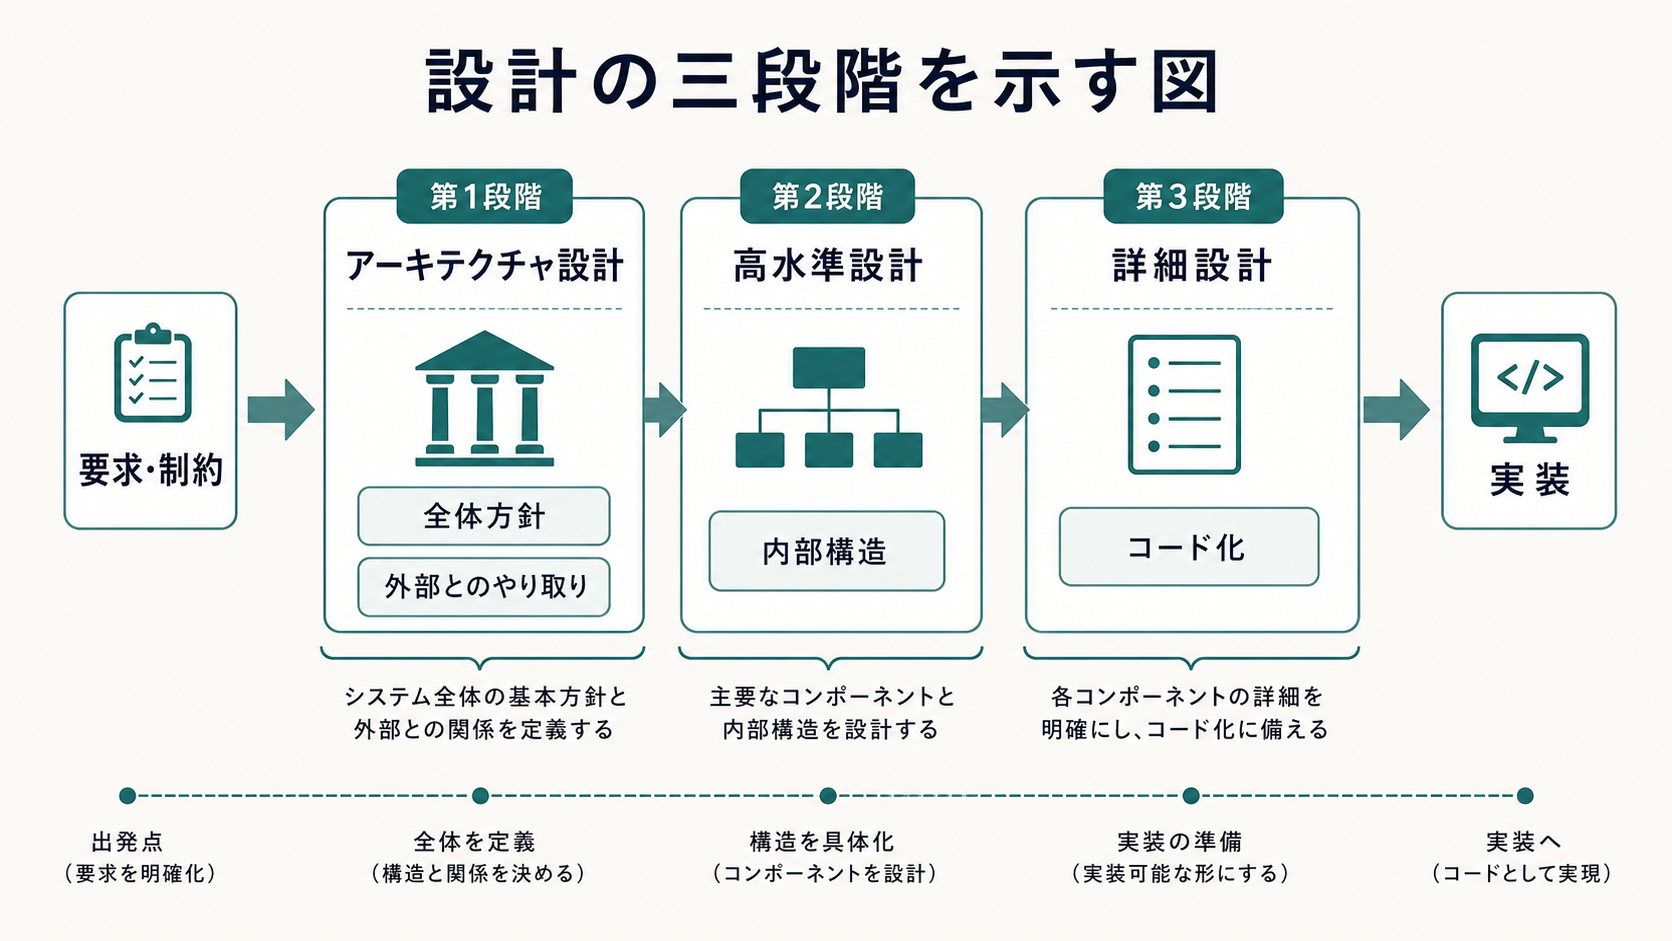
\includegraphics[width=0.96\linewidth]{assets/generated_figures/ch03/fig-ch03-05.png}}{\fbox{\parbox[c][48mm][c]{0.9\linewidth}{\centering 画像生成待ち\\設計の三段階を示す図}}}
\caption{設計の三段階を示す図}
\label{fig:ch03-05}
\end{figure}
